
\chapter{Introduction to Natural Language Processing}

\section{Applying Machine Learning to Text}

\definitionblock[Text]{
    A \textbf{text} is a sequence of symbols, which can be characters, words, or sentences. It belongs to an alphabet A:
    \begin{center}
        $x \in A^*$
    \end{center} 
    where $A^*$ is the set of all possible strings of symbols from A, in modern times UTF-16 (including emojis).
}

A dataset X of texts is called a \textbf{corpus}. A single text $x_i$ is called a \textbf{document}.

\subsection{Sentiment Analysis}

The goal is to gain insights about the sentiments an author was feeling while authoring a document.
This is a supervised learning problem, where the input is a document and the output is a sentiment label.

Preprocessing is essential, to obtain multivariate observations from the text. 

\begin{center}
    \begin{figure}[H]
        \centering
        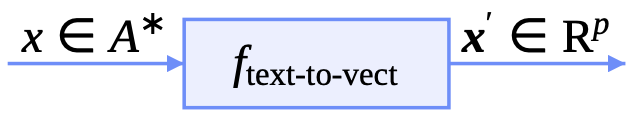
\includegraphics[width=0.4\textwidth]{assets/fig39.png}
        \caption{Sentiment Analysis}
    \end{figure}
\end{center}

A \textbf{Bag of Words (BOW)} is a representation of text that describes the occurrence of words within a document. It involves two steps:
\begin{enumerate}
    \item Tokenization: splitting the text into words
    \item Counting: counting the occurrences of each word
\end{enumerate}

Common preprocessing steps here are:
\begin{itemize}
    \item Lowercasing
    \item Removing punctuation
    \item Removing stop words
    \item Stemming (reducing words to their root form)
\end{itemize}

The problem of BOW is that it tends to prefer words that are frequent in the corpus, but not necessarily informative.
For this reason we can use \textbf{TF-IDF} (Term Frequency-Inverse Document Frequency), which is a measure of how important a word is to a document in a collection or corpus.

It is obtained by multiplying the term frequency (TF) by the inverse document frequency (IDF):
\begin{center}
    $tfidf(t, d, D) = tf(t, d) \cdot idf(t, D)$
\end{center}

Where:
\begin{itemize}
    \item $tf(t, d)$ is the frequency of term t in document d
    \item $idf(t, D)$ is the logarithm of the ratio of the total number of documents in the corpus and the number of documents where the term t appears
    \item $D$ is the corpus
    \item $t$ is the term
    \item $d$ is the document
    \item $tfidf(t, d, D)$ is the TF-IDF score of term t in document d
\end{itemize}

Since with BOW, $p = |W|$, dimensional reduction is often necessary. Common practices are:
\begin{itemize}
    \item use a very small dictionary
    \item learn a small dictionary on the learning data 
    \item use tf-idf and get k most important words
    \item use a dimensionality reduction technique
\end{itemize}

Also \textbf{ordering} is very important:
\begin{itemize}
    \item ngrams $\to$ Instead of considering word frequencies (or occurrences, or tf-idf ), consider the frequencies of short sequences of up-to words
    \item part of speech tagging $\to$ Instead of considering words, consider the frequencies of parts of speech
\end{itemize}

